% !TEX root = ../Documentation.tex

\section{Test Report}
\label{sec:tests}

\subsection{Test suite}
  Together with the new parser, a test suite has been developed.
  This test suite has been used to verify the performance and correctness of the new parser.
  The source code can be found in the folder \texttt{src/Database/Design/Ampersand/Test} within the Ampersand repository.

  The test suite runs in three steps, which are depicted in \autoref{fig:TestModules}.
  Each of the modules are described in the following subsection.
  %
  \begin{figure}[ht]%
    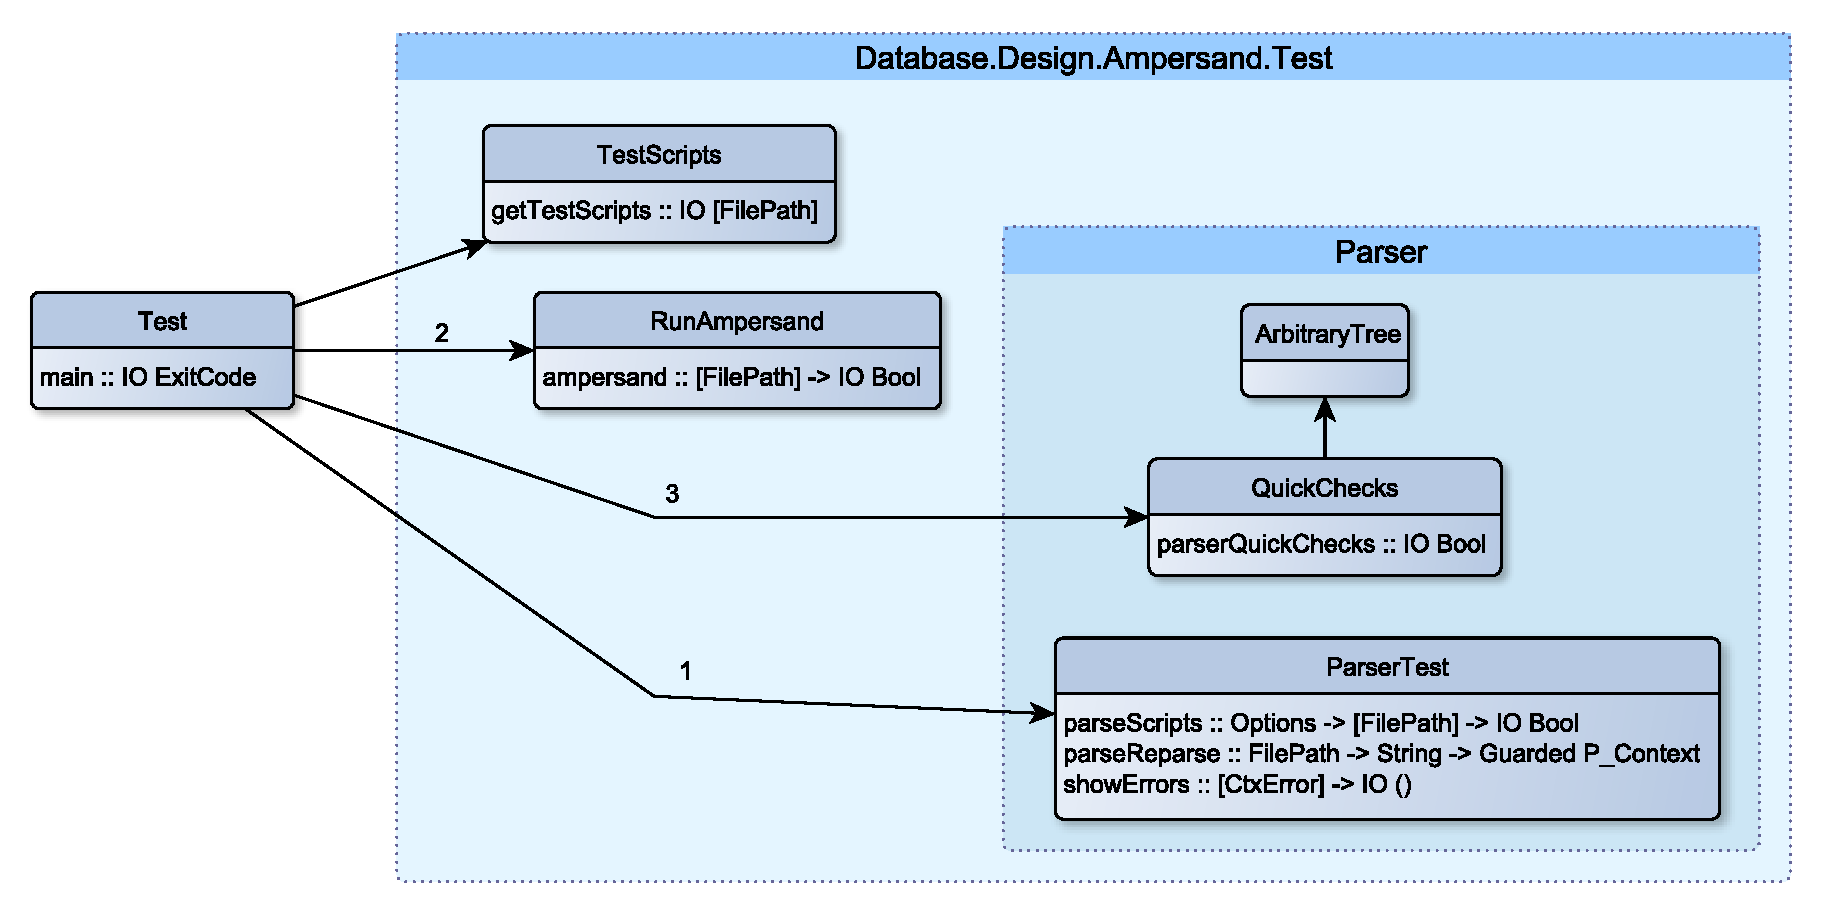
\includegraphics[width=\columnwidth]{figures/TestModules.pdf}
    \caption{Test suite modules with their exported functions}
    \label{fig:TestModules}
  \end{figure}%

  \subsubsection{Modules}
  \label{subsec:modules}
  In this section a short description of each module is given:%
  %
  \begin{description}
    \item[Test] This module contains a main method that can be executed to run the test suite.
      The \texttt{main} function calls each of the other modules in sequence, stopping if any of them returns \texttt{False}.
    
    \item[TestScripts] This module retrieves a list of scripts that can be used for the different tests.
      It searches for tests within the folder \texttt{ArchitectureAndDesign}, and contains a list of scripts from the \texttt{ampersand-models} repository, that can be changed at a later moment if wished.
      Note that all the ADL-scripts listed in this section must be correct for the parser and the type checker.
    
    \item[ParserTest] This module receives a list of 
    
    \item[RunAmpersand]
    
    \item[QuickChecks]
    
    \item[ArbitraryTree]
  \end{description}

  \subsubsection{Parser testing}
  TODO: Describe the parser tests.

  \subsubsection{Pretty printing}
  TODO: Describe the tests with pretty printing + parsing.

  \subsubsection{Chain test}
  TODO: Describe the chain tests done with the model scripts.

\subsection{Errors}
  Since evaluating the quality of error messages is manual work, the errors have not been included in the test suite.
  TODO: Give Maarten's findings on how the errors have improved. Maybe the tables should be an attachment, but the summary should be here.

\subsection{Next steps}
  TODO: Give suggestions on how to improve the tests.
  It may be pertinent to add the parser to Cabal testing and integrating the Sentinel jobs into the test suite.